\documentclass[tikz]{standalone}
\begin{document}

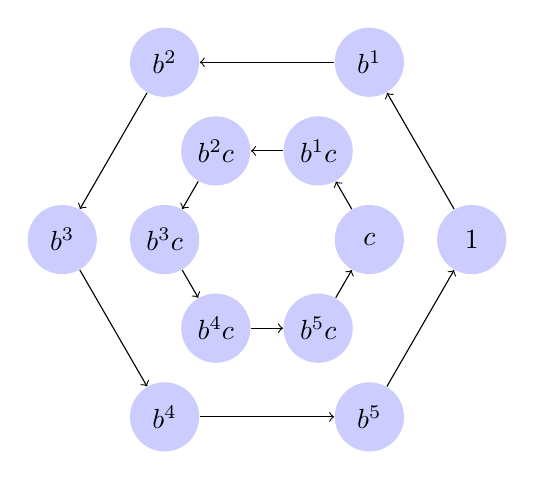
\begin{tikzpicture}
% Radius of regular polygons
\newdimen\Radi
\Radi=1.3cm
        \foreach \x/\n in {1/a,2/b,3/c,4/d,5/e} { 
                \node[circle,minimum size=2.5em,fill=blue!20] ({\n}0) at ({\Radi*cos(60*\x)},{\Radi*sin(60*\x)}) {\(b^{\x}c\)};
                \node[circle,minimum size=2.5em,fill=blue!20] ({\n}1) at ({2*\Radi*cos(60*\x)},{2*\Radi*sin(60*\x)}) {\(b^{\x}\)};
		}
        \node[circle,minimum size=2.5em,fill=blue!20] ({f}0) at ({\Radi},{0}) {\(c\)};
        \node[circle,minimum size=2.5em,fill=blue!20] ({f}1) at ({2*\Radi},{0}) {\(1\)};                  
		\foreach \from/\to in {a/b,b/c,c/d,d/e,e/f,f/a} {
		\draw [->] ({\from}0) -- ({\to}0);
		\draw [->] ({\from}1) -- ({\to}1);
		}
\end{tikzpicture}
\end{document}
